\label{chap:data}
Um Daten von übermüdeten Fahrern zu erhalten, kann natürlich kein Versuch im Straßenverkehr durchgeführt werden. Die Fremd- und Eigengefährdung wäre einfach zu groß. Darum fanden die Versuche in einer Simulationsumgebung statt. Für das Experiment wird im Fahrsimulator eine Nacht-Autobahnfahrt simuliert. Verschiedene Studien \cite{Engstrom_2322937}, \cite{Horne_1757738} legen nahe, dass sich  Simulationen zwar von der Realität unterscheiden, dass jedoch die Ergebnisse trotzdem valide und brauchbar sind.

Für den Versuch werden neben den rohen EEG Signalen, auch die Fahrzeugdaten, sowie die Simulation und der Fahrer aufgenommen. Weiterhin kann der Versuchsleiter auch Besonderheiten protokollieren (Abb. \ref{fig:experiment}).

\begin{figure}[h] 
  \begin{center}
    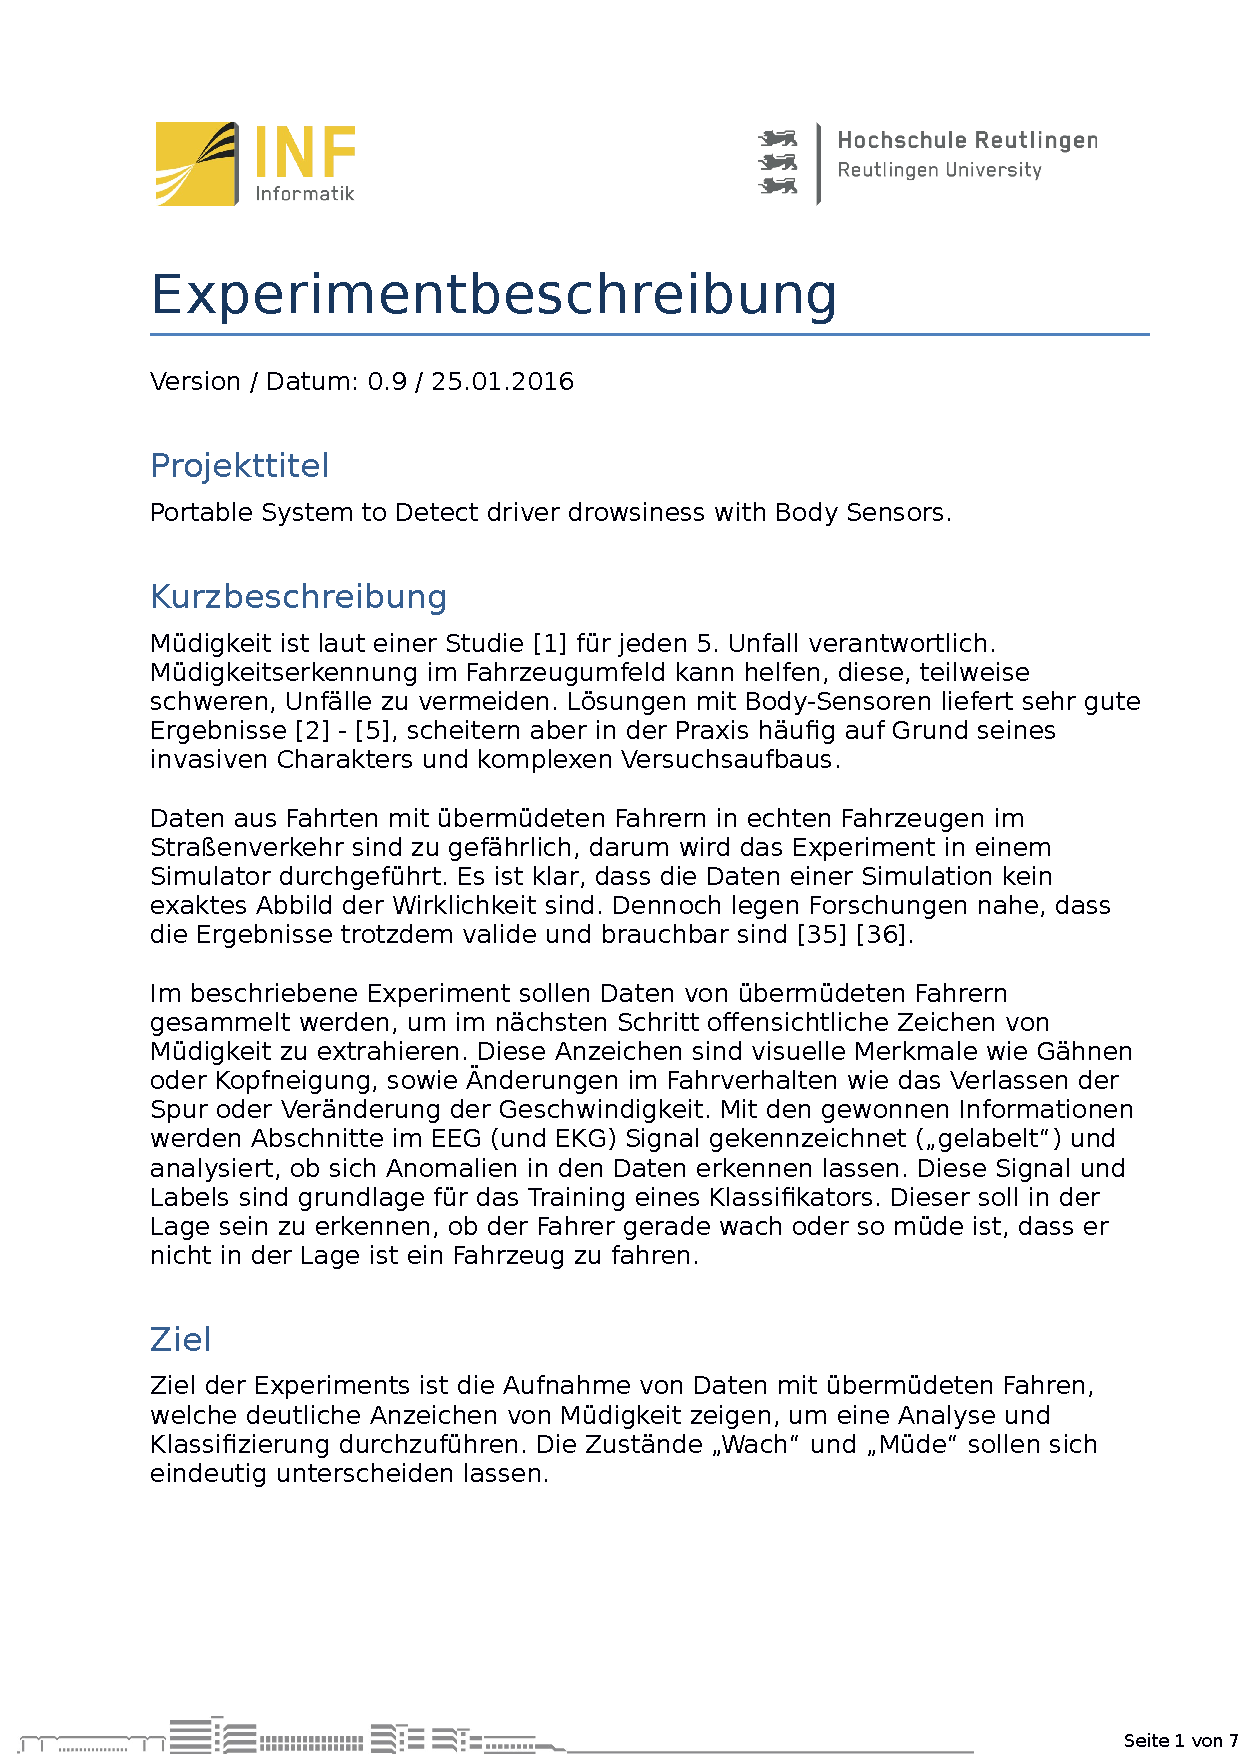
\includegraphics[width=\columnwidth]{experiment}
    \caption[Versuchsaufbau Experiment]{Der Versuchsaufbau für die Erkennung von Müdigkeit mit den Datenströmen aus der Fahrerkabine zur Testüberwachung. \label{fig:experiment}}
  \end{center}
\end{figure}

Im Versuch sollte der Fahrer eindeutige Anzeichen von Müdigkeit zeigen. Dies kann durch verschiedene Versuchsparameter begünstigt werden. So zeigt eine Studie, dass Unfälle meist zwischen 2:00 - 6:00, sowie 14:00 - 16:00 Uhr passieren \cite{Horne_1757738}. Auch die Schlafmenge von weniger als 6 Stunden in der Nacht vor dem Experiment erhöht die Chance auf Anzeichen \cite{Engstrom_2322937}. Das Geschlecht oder Alter der Probanden ist nicht relevant. Vor dem Experiment sollten jedoch keine Drogen, Alkohol oder Kaffee eingenommen werden. Ein Führerschein ist von Vorteil, aber nicht zwingend notwendig.

Auch die Teststrecke (Abb. \ref{fig:drivingtask}) trägt zur Erhöhung der Müdigkeit bei. Monotone Autobahnfahrten die größtenteils geradeaus verlaufen, ohne andere Verkehrsteilnehmer und konstanter Geschwindigkeit führen eher zu einer Übermüdung. Nach diesen Kriterien wurde eine endlose zweispurige Autobahnkarte mit einer Geschwindigkeit von konstant 130Kmh erstellt. Sie spielt zudem Nachts und ist eher Dunkel gehalten, was besonders anstrengend für die Augen ist.

\begin{figure}[h] 
  \begin{center}
    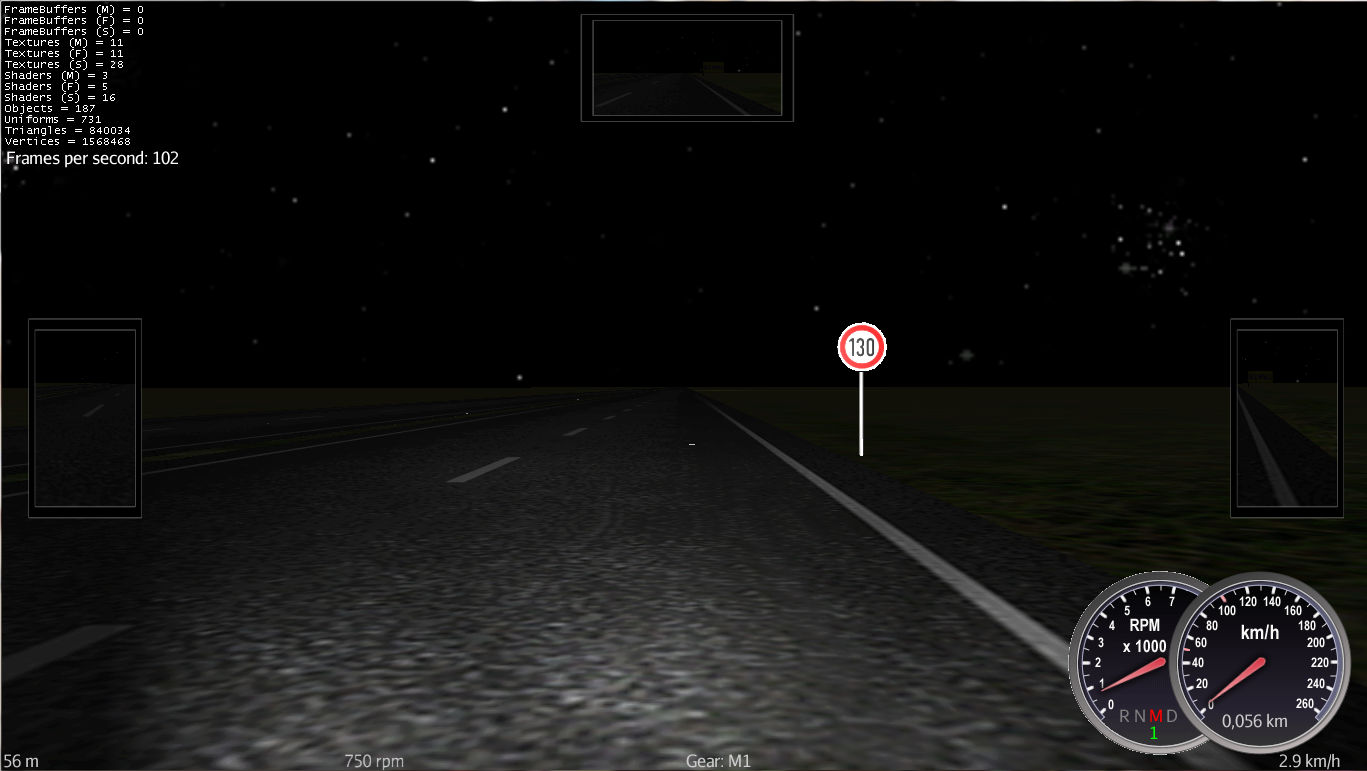
\includegraphics[width=0.75\columnwidth]{drivingtask}
    \caption[Driving Task Screenshot]{Die Autobahnkarte für den Versuch verläuft endlos geradeaus, Nachts und bei konstanter Geschwindigkeit. \label{fig:drivingtask}}
  \end{center}
\end{figure}

Für einen Versuch werden 40 Minuten angesetzt. Fünf Minuten werden für eine kurze Einführung, 30 Minuten für die Testfahrt und wieder fünf Minuten für eine kurze Einschätzung mit Fragebogen.

Anhand der aufgenommenen Daten werden nun Stellen gesucht, an denen die Testperson eindeutige Anzeichen von Müdigkeit zeigt. Eindeutig sind Verhaltensweisen wie häufiges Gähnen und Einnicken (Kopf fällt nach vorn) - Diese Merkmale werden häufig in CV-Ansätzen genutzt. 
Auch Verhaltensmerkmale wie, von der Spur abkommen und heftig Gegenlenken oder deutliche Veränderungen der Geschwindigkeit können Anzeichen für eine Unachtsamkeit wegen Müdigkeit sein.
Diese Stellen werden dann in den EEG Daten mit dem Label "`Müde"' markiert, alle anderen mit "`Wach"'. Die EEG Sequenzen können dann auf eindeutige Varianzen untersucht werden. Im nächsten Kapitel ist dies Thema der  Datenaufbereitung.